\documentclass{article}

\usepackage{etex}
\usepackage{amsmath}
\interdisplaylinepenalty=2500
\usepackage{amssymb,amsfonts,amsthm,mathrsfs,stmaryrd}
%\usepackage{geometry}
\usepackage{proof}
\usepackage{pst-all}
\usepackage[utf8]{inputenc}
\usepackage{bussproofs}
\usepackage[all]{xy}
\usepackage{graphicx}
% generated by Ott 0.24 from: lang.ott
\usepackage{ottlayout}
\usepackage{mathpartir}


\newcommand{\ottdrule}[4][]{{\displaystyle\frac{\begin{array}{l}#2\end{array}}{#3}\quad\ottdrulename{#4}}}
\newcommand{\ottusedrule}[1]{\[#1\]}
\newcommand{\ottpremise}[1]{ #1 \\}
\newenvironment{ottdefnblock}[3][]{ \framebox{\mbox{#2}} \quad #3 \\[0pt]}{}
\newenvironment{ottfundefnblock}[3][]{ \framebox{\mbox{#2}} \quad #3 \\[0pt]\begin{displaymath}\begin{array}{l}}{\end{array}\end{displaymath}}
\newcommand{\ottfunclause}[2]{ #1 \equiv #2 \\}
\newcommand{\ottnt}[1]{\mathit{#1}}
\newcommand{\ottmv}[1]{\mathit{#1}}
\newcommand{\ottkw}[1]{\mathbf{#1}}
\newcommand{\ottsym}[1]{#1}
\newcommand{\ottcom}[1]{\text{#1}}
\newcommand{\ottdrulename}[1]{\textsc{#1}}
\newcommand{\ottcomplu}[5]{\overline{#1}^{\,#2\in #3 #4 #5}}
\newcommand{\ottcompu}[3]{\overline{#1}^{\,#2<#3}}
\newcommand{\ottcomp}[2]{\overline{#1}^{\,#2}}
\newcommand{\ottgrammartabular}[1]{\begin{supertabular}{llcllllll}#1\end{supertabular}}
\newcommand{\ottmetavartabular}[1]{\begin{supertabular}{ll}#1\end{supertabular}}
\newcommand{\ottrulehead}[3]{$#1$ & & $#2$ & & & \multicolumn{2}{l}{#3}}
\newcommand{\ottprodline}[6]{& & $#1$ & $#2$ & $#3 #4$ & $#5$ & $#6$}
\newcommand{\ottfirstprodline}[6]{\ottprodline{#1}{#2}{#3}{#4}{#5}{#6}}
\newcommand{\ottlongprodline}[2]{& & $#1$ & \multicolumn{4}{l}{$#2$}}
\newcommand{\ottfirstlongprodline}[2]{\ottlongprodline{#1}{#2}}
\newcommand{\ottbindspecprodline}[6]{\ottprodline{#1}{#2}{#3}{#4}{#5}{#6}}
\newcommand{\ottprodnewline}{\\}
\newcommand{\ottinterrule}{\\[5.0mm]}
\newcommand{\ottafterlastrule}{\\}
\newcommand{\ottmetavars}{
\ottmetavartabular{
 $ \ottmv{termvar} ,\, \ottmv{x} ,\, \ottmv{f} $ &  \\
}}

\newcommand{\ottnat}{
\ottrulehead{\ottnt{nat}  ,\ \ottnt{n}  ,\ \ottnt{p}}{::=}{}\ottprodnewline
\ottfirstprodline{|}{\ottsym{0}} {\textsf{M}}{}{}{}\ottprodnewline
\ottprodline{|}{\ottsym{1}} {\textsf{M}}{}{}{}\ottprodnewline
\ottprodline{|}{\ottnt{n_{{\mathrm{1}}}}  \ottsym{+}  \ottnt{n_{{\mathrm{2}}}}} {\textsf{M}}{}{}{}\ottprodnewline
\ottprodline{|}{\sigma \, \ottmv{x}} {\textsf{M}}{}{}{}\ottprodnewline
\ottprodline{|}{ [\![  \ottnt{E}  ]\!]_{ \sigma } } {\textsf{M}}{}{}{}}

\newcommand{\ottstore}{
\ottrulehead{\ottnt{store}  ,\ \sigma}{::=}{}\ottprodnewline
\ottfirstprodline{|}{\sigma  \ottsym{[}  \ottmv{x}  \ottsym{:=}  \ottnt{n}  \ottsym{]}} {\textsf{M}}{}{}{}}

\newcommand{\ottexp}{
\ottrulehead{\ottnt{exp}  ,\ \ottnt{E}}{::=}{}\ottprodnewline
\ottfirstprodline{|}{\ottmv{x}}{}{}{}{}\ottprodnewline
\ottprodline{|}{\ottnt{E_{{\mathrm{1}}}}  \ottsym{+}  \ottnt{E_{{\mathrm{2}}}}}{}{}{}{}\ottprodnewline
\ottprodline{|}{\ottsym{(}  \ottnt{E}  \ottsym{)}} {\textsf{S}}{}{}{}}

\newcommand{\ottbexp}{
\ottrulehead{\ottnt{bexp}  ,\ \ottnt{B}}{::=}{}\ottprodnewline
\ottfirstprodline{|}{\ottnt{E_{{\mathrm{1}}}}  \ottsym{=}  \ottnt{E_{{\mathrm{2}}}}}{}{}{}{}\ottprodnewline
\ottprodline{|}{\ottnt{E_{{\mathrm{1}}}}  \ottsym{<}  \ottnt{E_{{\mathrm{2}}}}}{}{}{}{}}

\newcommand{\ottcmd}{
\ottrulehead{\ottnt{cmd}  ,\ \ottnt{C}}{::=}{}\ottprodnewline
\ottfirstprodline{|}{\ottkw{skip}}{}{}{}{}\ottprodnewline
\ottprodline{|}{\ottmv{x}  \ottsym{=}  \ottnt{E}}{}{}{}{}\ottprodnewline
\ottprodline{|}{\ottkw{assume} \, \ottnt{B}}{}{}{}{}\ottprodnewline
\ottprodline{|}{\ottnt{C_{{\mathrm{1}}}}  \ottsym{;}  \ottnt{C_{{\mathrm{2}}}}}{}{}{}{}\ottprodnewline
\ottprodline{|}{\ottkw{atomic} \, \ottnt{C}}{}{}{}{}\ottprodnewline
\ottprodline{|}{\ottkw{loop} \, \ottnt{C}}{}{}{}{}\ottprodnewline
\ottprodline{|}{ \mathbf{inloop}^{ \ottnt{p} }_{ \ottnt{C_{{\mathrm{2}}}} }( \ottnt{C_{{\mathrm{1}}}} ) }{}{}{}{}\ottprodnewline
\ottprodline{|}{\ottkw{break}}{}{}{}{}\ottprodnewline
\ottprodline{|}{ \ottnt{C_{{\mathrm{1}}}}  \parallel  \ottnt{C_{{\mathrm{2}}}} }{}{}{}{}\ottprodnewline
\ottprodline{|}{ \ottnt{C_{{\mathrm{1}}}}  \oplus  \ottnt{C_{{\mathrm{2}}}} }{}{}{}{}\ottprodnewline
\ottprodline{|}{\ottsym{(}  \ottnt{C}  \ottsym{)}} {\textsf{S}}{}{}{}}

\newcommand{\ottformula}{
\ottrulehead{\ottnt{formula}}{::=}{}\ottprodnewline
\ottfirstprodline{|}{\ottnt{judgement}}{}{}{}{}\ottprodnewline
\ottprodline{|}{\ottnt{n_{{\mathrm{1}}}}  \ottsym{=}  \ottnt{n_{{\mathrm{2}}}}} {\textsf{M}}{}{}{}\ottprodnewline
\ottprodline{|}{\ottnt{n_{{\mathrm{1}}}}  \ottsym{<}  \ottnt{n_{{\mathrm{2}}}}} {\textsf{M}}{}{}{}\ottprodnewline
\ottprodline{|}{\ottkw{True}} {\textsf{M}}{}{}{}\ottprodnewline
\ottprodline{|}{\ottkw{False}} {\textsf{M}}{}{}{}\ottprodnewline
\ottprodline{|}{ ( \ottnt{formula} ) } {\textsf{M}}{}{}{}\ottprodnewline
\ottprodline{|}{\ottnt{formula_{{\mathrm{1}}}}  \vee  \ottnt{formula_{{\mathrm{2}}}}} {\textsf{M}}{}{}{}\ottprodnewline
\ottprodline{|}{\ottnt{formula_{{\mathrm{1}}}}  \wedge  \ottnt{formula_{{\mathrm{2}}}}} {\textsf{M}}{}{}{}\ottprodnewline
\ottprodline{|}{ [\![  \ottnt{B}  ]\!]_{ \sigma } } {\textsf{M}}{}{}{}\ottprodnewline
\ottprodline{|}{ \textbf{aborts} \langle \ottnt{C} , \sigma , \ottnt{p} \rangle } {\textsf{M}}{}{}{}}

\newcommand{\ottterminals}{
\ottrulehead{\ottnt{terminals}}{::=}{}\ottprodnewline
\ottfirstprodline{|}{ \vee }{}{}{}{}\ottprodnewline
\ottprodline{|}{ \wedge }{}{}{}{}\ottprodnewline
\ottprodline{|}{ \leq }{}{}{}{}}

\newcommand{\ottedenotXXfuns}{
\ottrulehead{\ottnt{edenot\_funs}}{::=}{}\ottprodnewline
\ottfirstprodline{|}{ [\![  \ottnt{E}  ]\!]_{ \sigma } }{}{}{}{}\ottprodnewline
\ottprodline{|}{ [\![  \ottnt{B}  ]\!]_{ \sigma } }{}{}{}{}}

\newcommand{\ottabortXXfuns}{
\ottrulehead{\ottnt{abort\_funs}}{::=}{}\ottprodnewline
\ottfirstprodline{|}{ \textbf{aborts} \langle \ottnt{C} , \sigma , \ottnt{p} \rangle }{}{}{}{}}

\newcommand{\ottOpSemJudg}{
\ottrulehead{\ottnt{OpSemJudg}}{::=}{}\ottprodnewline
\ottfirstprodline{|}{ \langle  \ottnt{C}  ,  \sigma  ,  \ottnt{p}  \rangle \to \langle  \ottnt{C'}  ,  \sigma' , \ottnt{p'}  \rangle }{}{}{}{\ottcom{small step}}}

\newcommand{\ottjudgement}{
\ottrulehead{\ottnt{judgement}}{::=}{}\ottprodnewline
\ottfirstprodline{|}{\ottnt{OpSemJudg}}{}{}{}{}}

\newcommand{\ottuserXXsyntax}{
\ottrulehead{\ottnt{user\_syntax}}{::=}{}\ottprodnewline
\ottfirstprodline{|}{\ottmv{termvar}}{}{}{}{}\ottprodnewline
\ottprodline{|}{\ottnt{nat}}{}{}{}{}\ottprodnewline
\ottprodline{|}{\ottnt{store}}{}{}{}{}\ottprodnewline
\ottprodline{|}{\ottnt{exp}}{}{}{}{}\ottprodnewline
\ottprodline{|}{\ottnt{bexp}}{}{}{}{}\ottprodnewline
\ottprodline{|}{\ottnt{cmd}}{}{}{}{}\ottprodnewline
\ottprodline{|}{\ottnt{formula}}{}{}{}{}\ottprodnewline
\ottprodline{|}{\ottnt{terminals}}{}{}{}{}}

\newcommand{\ottgrammar}{\ottgrammartabular{
\ottnat\ottinterrule
\ottstore\ottinterrule
\ottexp\ottinterrule
\ottbexp\ottinterrule
\ottcmd\ottinterrule
\ottformula\ottinterrule
\ottterminals\ottinterrule
\ottedenotXXfuns\ottinterrule
\ottabortXXfuns\ottinterrule
\ottOpSemJudg\ottinterrule
\ottjudgement\ottinterrule
\ottuserXXsyntax\ottafterlastrule
}}

% defnss
% fundefns edenot_funs
% fundefn edenot

\newcommand{\ottfundefnedenot}[1]{\begin{ottfundefnblock}[#1]{$ [\![  \ottnt{E}  ]\!]_{ \sigma } $}{}
\ottfunclause{ [\![  \ottmv{x}  ]\!]_{ \sigma } }{\sigma \, \ottmv{x}}%
\ottfunclause{ [\![  \ottnt{E_{{\mathrm{1}}}}  \ottsym{+}  \ottnt{E_{{\mathrm{2}}}}  ]\!]_{ \sigma } }{ [\![  \ottnt{E_{{\mathrm{1}}}}  ]\!]_{ \sigma }   \ottsym{+}   [\![  \ottnt{E_{{\mathrm{2}}}}  ]\!]_{ \sigma } }%
\end{ottfundefnblock}}


% fundefn bdenot

\newcommand{\ottfundefnbdenot}[1]{\begin{ottfundefnblock}[#1]{$ [\![  \ottnt{B}  ]\!]_{ \sigma } $}{}
\ottfunclause{ [\![  \ottnt{E_{{\mathrm{1}}}}  \ottsym{=}  \ottnt{E_{{\mathrm{2}}}}  ]\!]_{ \sigma } }{ [\![  \ottnt{E_{{\mathrm{1}}}}  ]\!]_{ \sigma }   \ottsym{=}   [\![  \ottnt{E_{{\mathrm{2}}}}  ]\!]_{ \sigma } }%
\ottfunclause{ [\![  \ottnt{E_{{\mathrm{1}}}}  \ottsym{<}  \ottnt{E_{{\mathrm{2}}}}  ]\!]_{ \sigma } }{ [\![  \ottnt{E_{{\mathrm{1}}}}  ]\!]_{ \sigma }   \ottsym{<}   [\![  \ottnt{E_{{\mathrm{2}}}}  ]\!]_{ \sigma } }%
\end{ottfundefnblock}}


\newcommand{\ottfundefnsedenotXXfuns}{
\ottfundefnedenot{}
\ottfundefnbdenot{}}

% fundefns abort_funs
% fundefn aborts

\newcommand{\ottfundefnaborts}[1]{\begin{ottfundefnblock}[#1]{$ \textbf{aborts} \langle \ottnt{C} , \sigma , \ottnt{p} \rangle $}{}
\ottfunclause{ \textbf{aborts} \langle \ottnt{C_{{\mathrm{1}}}}  \ottsym{;}  \ottnt{C_{{\mathrm{2}}}} , \sigma , \ottnt{p} \rangle }{ \textbf{aborts} \langle \ottnt{C_{{\mathrm{1}}}} , \sigma , \ottnt{p} \rangle }%
\ottfunclause{ \textbf{aborts} \langle  \ottnt{C_{{\mathrm{1}}}}  \parallel  \ottnt{C_{{\mathrm{2}}}}  , \sigma , \ottnt{p} \rangle }{ \textbf{aborts} \langle \ottnt{C_{{\mathrm{1}}}} , \sigma , \ottnt{p} \rangle   \vee   \textbf{aborts} \langle \ottnt{C_{{\mathrm{2}}}} , \sigma , \ottnt{p} \rangle }%
\ottfunclause{ \textbf{aborts} \langle  \mathbf{inloop}^{ \ottnt{p'} }_{ \ottnt{C} }( \ottkw{skip} )  , \sigma , \ottnt{p} \rangle }{\ottnt{p'}  \ottsym{<}  \ottnt{p}}%
\ottfunclause{ \textbf{aborts} \langle \ottnt{C} , \sigma , \ottnt{p} \rangle }{\ottkw{False}}%
\ottfunclause{ \textbf{aborts} \langle \ottkw{atomic} \, \ottnt{C} , \sigma , \ottnt{p} \rangle }{ \textbf{aborts} \langle \ottnt{C} , \sigma , \ottnt{p} \rangle }%
\end{ottfundefnblock}}


\newcommand{\ottfundefnsabortXXfuns}{
\ottfundefnaborts{}}

% defns OpSemJudg
%% defn step
\newcommand{\ottdruleSassign}[1]{\ottdrule[#1]{%
}{
 \langle  \ottmv{x}  \ottsym{=}  \ottnt{E}  ,  \sigma  ,  \ottnt{p}  \rangle \to \langle  \ottkw{skip}  ,  \sigma  \ottsym{[}  \ottmv{x}  \ottsym{:=}   [\![  \ottnt{E}  ]\!]_{ \sigma }   \ottsym{]} , \ottnt{p}  \ottsym{+}  \ottsym{1}  \rangle }{%
{\ottdrulename{Sassign}}{}%
}}


\newcommand{\ottdruleSseqI}[1]{\ottdrule[#1]{%
\ottpremise{ \langle  \ottnt{C_{{\mathrm{1}}}}  ,  \sigma  ,  \ottnt{p}  \rangle \to \langle  \ottnt{C'_{{\mathrm{1}}}}  ,  \sigma' , \ottnt{p'}  \rangle }%
}{
 \langle  \ottnt{C_{{\mathrm{1}}}}  \ottsym{;}  \ottnt{C_{{\mathrm{2}}}}  ,  \sigma  ,  \ottnt{p}  \rangle \to \langle  \ottnt{C'_{{\mathrm{1}}}}  \ottsym{;}  \ottnt{C_{{\mathrm{2}}}}  ,  \sigma' , \ottnt{p'}  \rangle }{%
{\ottdrulename{SseqI}}{}%
}}


\newcommand{\ottdruleSseqII}[1]{\ottdrule[#1]{%
}{
 \langle  \ottkw{skip}  \ottsym{;}  \ottnt{C_{{\mathrm{2}}}}  ,  \sigma  ,  \ottnt{p}  \rangle \to \langle  \ottnt{C_{{\mathrm{2}}}}  ,  \sigma , \ottnt{p}  \rangle }{%
{\ottdrulename{SseqII}}{}%
}}


\newcommand{\ottdruleSassume}[1]{\ottdrule[#1]{%
\ottpremise{ [\![  \ottnt{B}  ]\!]_{ \sigma } }%
}{
 \langle  \ottkw{assume} \, \ottnt{B}  ,  \sigma  ,  \ottnt{p}  \rangle \to \langle  \ottkw{skip}  ,  \sigma , \ottnt{p}  \rangle }{%
{\ottdrulename{Sassume}}{}%
}}


\newcommand{\ottdruleSparI}[1]{\ottdrule[#1]{%
\ottpremise{ \langle  \ottnt{C_{{\mathrm{1}}}}  ,  \sigma  ,  \ottnt{p}  \rangle \to \langle  \ottnt{C'_{{\mathrm{1}}}}  ,  \sigma' , \ottnt{p'}  \rangle }%
}{
 \langle   \ottnt{C_{{\mathrm{1}}}}  \parallel  \ottnt{C_{{\mathrm{2}}}}   ,  \sigma  ,  \ottnt{p}  \rangle \to \langle   \ottnt{C'_{{\mathrm{1}}}}  \parallel  \ottnt{C_{{\mathrm{2}}}}   ,  \sigma' , \ottnt{p'}  \rangle }{%
{\ottdrulename{SparI}}{}%
}}


\newcommand{\ottdruleSparII}[1]{\ottdrule[#1]{%
\ottpremise{ \langle  \ottnt{C_{{\mathrm{2}}}}  ,  \sigma  ,  \ottnt{p}  \rangle \to \langle  \ottnt{C'_{{\mathrm{2}}}}  ,  \sigma' , \ottnt{p'}  \rangle }%
}{
 \langle   \ottnt{C_{{\mathrm{1}}}}  \parallel  \ottnt{C_{{\mathrm{2}}}}   ,  \sigma  ,  \ottnt{p}  \rangle \to \langle   \ottnt{C_{{\mathrm{1}}}}  \parallel  \ottnt{C'_{{\mathrm{2}}}}   ,  \sigma' , \ottnt{p'}  \rangle }{%
{\ottdrulename{SparII}}{}%
}}


\newcommand{\ottdruleSparIII}[1]{\ottdrule[#1]{%
}{
 \langle   \ottkw{skip}  \parallel  \ottkw{skip}   ,  \sigma  ,  \ottnt{p}  \rangle \to \langle  \ottkw{skip}  ,  \sigma , \ottnt{p}  \rangle }{%
{\ottdrulename{SparIII}}{}%
}}


\newcommand{\ottdruleSloopEnter}[1]{\ottdrule[#1]{%
}{
 \langle  \ottkw{loop} \, \ottnt{C}  ,  \sigma  ,  \ottnt{p}  \rangle \to \langle   \mathbf{inloop}^{ \ottnt{p} }_{ \ottnt{C} }( \ottnt{C} )   ,  \sigma , \ottnt{p}  \rangle }{%
{\ottdrulename{SloopEnter}}{}%
}}


\newcommand{\ottdruleSloopSeq}[1]{\ottdrule[#1]{%
\ottpremise{ \langle  \ottnt{C_{{\mathrm{1}}}}  ,  \sigma  ,  \ottnt{p}  \rangle \to \langle  \ottnt{C'_{{\mathrm{1}}}}  ,  \sigma' , \ottnt{p'}  \rangle }%
}{
 \langle   \mathbf{inloop}^{ \ottnt{p_{{\mathrm{0}}}} }_{ \ottnt{C} }( \ottnt{C_{{\mathrm{1}}}} )   ,  \sigma  ,  \ottnt{p}  \rangle \to \langle   \mathbf{inloop}^{ \ottnt{p_{{\mathrm{0}}}} }_{ \ottnt{C} }( \ottnt{C'_{{\mathrm{1}}}} )   ,  \sigma , \ottnt{p}  \rangle }{%
{\ottdrulename{SloopSeq}}{}%
}}


\newcommand{\ottdruleSloopBreakI}[1]{\ottdrule[#1]{%
}{
 \langle   \mathbf{inloop}^{ \ottnt{p_{{\mathrm{0}}}} }_{ \ottnt{C} }( \ottkw{break} )   ,  \sigma  ,  \ottnt{p}  \rangle \to \langle  \ottkw{skip}  ,  \sigma , \ottnt{p}  \ottsym{+}  \ottsym{1}  \rangle }{%
{\ottdrulename{SloopBreakI}}{}%
}}


\newcommand{\ottdruleSloopBreakII}[1]{\ottdrule[#1]{%
}{
 \langle   \mathbf{inloop}^{ \ottnt{p_{{\mathrm{0}}}} }_{ \ottnt{C} }( \ottkw{break}  \ottsym{;}  \ottnt{C_{{\mathrm{1}}}} )   ,  \sigma  ,  \ottnt{p}  \rangle \to \langle  \ottkw{skip}  ,  \sigma , \ottnt{p}  \ottsym{+}  \ottsym{1}  \rangle }{%
{\ottdrulename{SloopBreakII}}{}%
}}


\newcommand{\ottdruleSloopAssert}[1]{\ottdrule[#1]{%
\ottpremise{\ottnt{p_{{\mathrm{0}}}}  \ottsym{<}  \ottnt{p}}%
}{
 \langle   \mathbf{inloop}^{ \ottnt{p_{{\mathrm{0}}}} }_{ \ottnt{C} }( \ottkw{skip} )   ,  \sigma  ,  \ottnt{p}  \rangle \to \langle   \mathbf{inloop}^{ \ottnt{p} }_{ \ottnt{C} }( \ottnt{C} )   ,  \sigma , \ottnt{p}  \rangle }{%
{\ottdrulename{SloopAssert}}{}%
}}


\newcommand{\ottdruleSatom}[1]{\ottdrule[#1]{%
\ottpremise{ \langle  \ottnt{C}  ,  \sigma  ,  \ottnt{p}  \rangle \to \langle  \ottkw{skip}  ,  \sigma' , \ottnt{p'}  \rangle }%
}{
 \langle  \ottkw{atomic} \, \ottnt{C}  ,  \sigma  ,  \ottnt{p}  \rangle \to \langle  \ottkw{skip}  ,  \sigma' , \ottnt{p'}  \rangle }{%
{\ottdrulename{Satom}}{}%
}}


\newcommand{\ottdruleSnondetI}[1]{\ottdrule[#1]{%
}{
 \langle   \ottnt{C_{{\mathrm{1}}}}  \oplus  \ottnt{C_{{\mathrm{2}}}}   ,  \sigma  ,  \ottnt{p}  \rangle \to \langle  \ottnt{C_{{\mathrm{1}}}}  ,  \sigma , \ottnt{p}  \rangle }{%
{\ottdrulename{SnondetI}}{}%
}}


\newcommand{\ottdruleSnondetII}[1]{\ottdrule[#1]{%
}{
 \langle   \ottnt{C_{{\mathrm{1}}}}  \oplus  \ottnt{C_{{\mathrm{2}}}}   ,  \sigma  ,  \ottnt{p}  \rangle \to \langle  \ottnt{C_{{\mathrm{2}}}}  ,  \sigma , \ottnt{p}  \rangle }{%
{\ottdrulename{SnondetII}}{}%
}}

\newcommand{\ottdefnstep}[1]{\begin{ottdefnblock}[#1]{$ \langle  \ottnt{C}  ,  \sigma  ,  \ottnt{p}  \rangle \to \langle  \ottnt{C'}  ,  \sigma' , \ottnt{p'}  \rangle $}{\ottcom{small step}}
\ottusedrule{\ottdruleSassign{}}
\ottusedrule{\ottdruleSseqI{}}
\ottusedrule{\ottdruleSseqII{}}
\ottusedrule{\ottdruleSassume{}}
\ottusedrule{\ottdruleSparI{}}
\ottusedrule{\ottdruleSparII{}}
\ottusedrule{\ottdruleSparIII{}}
\ottusedrule{\ottdruleSloopEnter{}}
\ottusedrule{\ottdruleSloopSeq{}}
\ottusedrule{\ottdruleSloopBreakI{}}
\ottusedrule{\ottdruleSloopBreakII{}}
\ottusedrule{\ottdruleSloopAssert{}}
\ottusedrule{\ottdruleSatom{}}
\ottusedrule{\ottdruleSnondetI{}}
\ottusedrule{\ottdruleSnondetII{}}
\end{ottdefnblock}}


\newcommand{\ottdefnsOpSemJudg}{
\ottdefnstep{}}

\newcommand{\ottdefnss}{
\ottfundefnsedenotXXfuns
\ottfundefnsabortXXfuns
\ottdefnsOpSemJudg
}

\newcommand{\ottall}{\ottmetavars\\[0pt]
\ottgrammar\\[5.0mm]
\ottdefnss}


\renewcommand{\ottmetavartabular}[1]{\begin{supertabular}{ll}#1\end{supertabular}}
\renewcommand{\ottgrammartabular}[1]{\begin{description} #1 \end{description}}
\renewcommand{\ottrulehead}[3]{\item[$#1$ $#2$] }
\renewcommand{\ottfirstprodline}[6]{$#2$}
\renewcommand{\ottprodline}[6]{\ifthenelse{\equal{#3}{}}{ $|$~\hbox{$#2$}}{}}
\renewcommand{\ottbindspecprodline}[6]{}
\renewcommand{\ottprodnewline}{}
\renewcommand{\ottinterrule}{ \par }
\renewcommand{\ottafterlastrule}{}

%\renewenvironment{ottfundefnblock}[3][]{
%  \begin{displaymath}\begin{array}{l@{~}c@{~}l}}
%  {\end{array}\end{displaymath}}
\renewenvironment{ottfundefnblock}[3][]{
  \framebox{\mbox{#2} } \quad #3 \\[0pt]\begin{displaymath}\begin{array}{l@{~}c@{~}l}}
  {\end{array}\end{displaymath}}
\renewcommand{\ottfunclause}[2]{ #1 &\equiv& #2 \\}

%% Use Rok's package for type-setting rules

\renewcommand{\ottpremise}[1]{\premiseSTY{#1} }
\renewcommand{\ottdrule}[4][]{\druleSTY[#1]{#2}{#3}{#4} }
\ottstyledefaults{premiselayout=justify,premisenamelayout=none}

%% and Didier Remy's one for packing them up tightly.

\renewcommand{\ottusedrule}[1]{ #1 \and }
\renewenvironment{ottdefnblock}[3][]{
%  \par\noindent \framebox{\mbox{#2} } \quad #3 \\
  \begin{mathparpagebreakable}
    }
  {\end{mathparpagebreakable}\par}




\newtheorem{defi}{Definition}
\newtheorem{theorem}{Theorem}[section]
\newtheorem{lemma}[theorem]{Lemma}

\CompileMatrices
\UseComputerModernTips

\renewcommand{\ttdefault}{cmtt}

% \title{\Large \bf Separation Logic in the Presence of Garbage Collection}
% \author{
% \IEEEauthorblockN{\large Chung-Kil Hur \qquad Derek Dreyer \qquad Viktor Vafeiadis} \\
% \IEEEauthorblockA{Max Planck Institute for Software Systems (MPI-SWS) \\ 
% \cd{\{gil,dreyer,viktor\}@mpi-sws.org}}
% }


\title{Proving Lock-Freedom Easily}

\author{
Wei Li \and Xiao Jia \and Viktor Vafeiadis
}

\begin{document}

\maketitle

\begin{abstract}
We present a new way for proving lock-freedom automatically.
\end{abstract}

%-----------------------------------------------------------------------------
\section{Introduction}
\label{sec:intro}
%-----------------------------------------------------------------------------
A non-blocking data structure should guarantee certain \textit{liveness properties}, which are ensured by progress conditions such as obstruction-freedom, lock-freedom, and wait-freedom. The strongest of these properties is wait-freedom, which requires each thread to make progress whenever it is scheduled for a sufficient number of steps, independently of other concurrently executing threads. Such behavior is indeed desirable, but this requirement is very strong and often results in a complicated and inefficient programs. Lock-freedom requires that when the program threads are run sufficiently long, at least one of the threads make progress. This requirement ensures that the program as a whole makes progress and is never blocked. Lock-free algorithms are known for various tasks and are often efficient. Obstruction freedom is the weakest requirement, stating that progress is only guaranteed if we let one of the program threads run in isolation sufficiently long. In this paper we concentrate on lock-freedom, which provides a strong progress guarantee and allows for efficient implementations in practice.

\begin{figure}
    \centering
    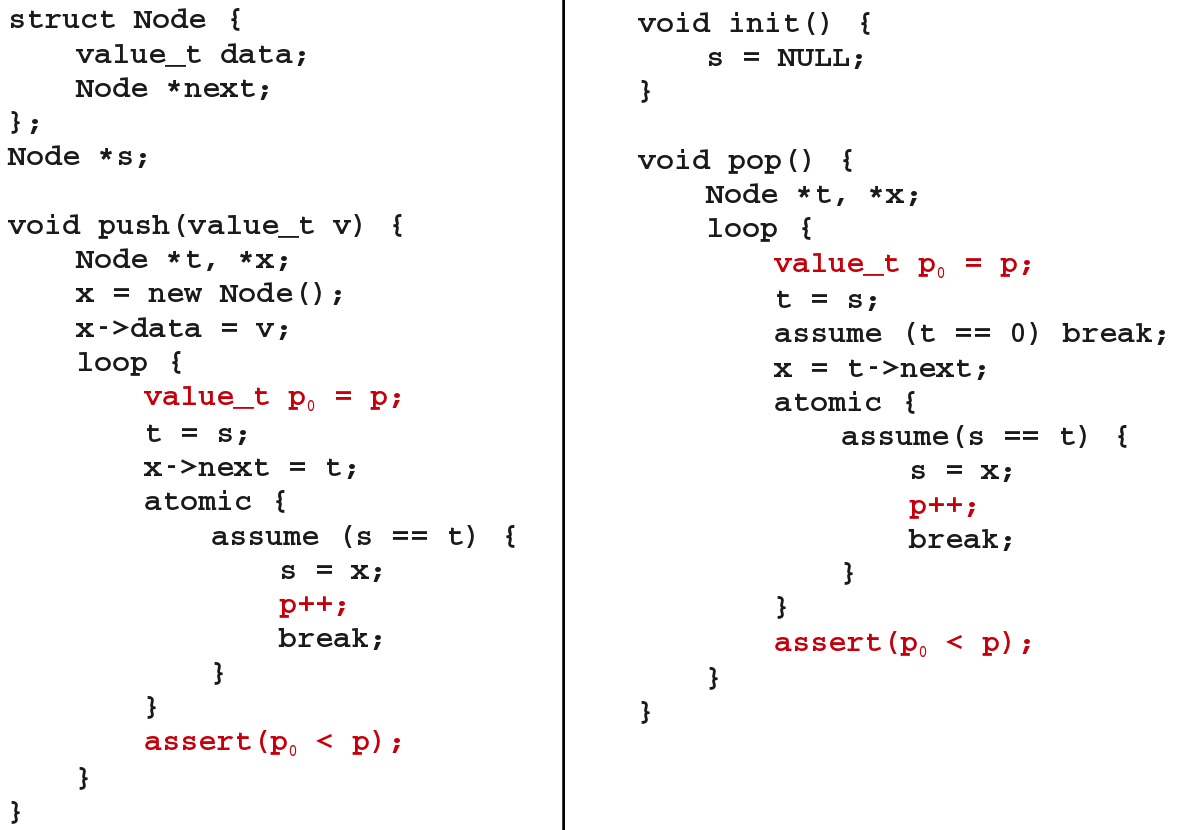
\includegraphics[width=0.7\textwidth]{treiber.png}
    \caption{Treiber's non-blocking stack with ghost variable $p$}
    \label{fig:treiber}
\end{figure}

We use Treiber's stack example to illustrate the method that can prove lock-free easily. A shared ghost variable $p$ is introduced to the original implemnentation of Treiber's stack, which will be incremented after each $break$, as is shown in Figure ~\ref{fig:treiber}. Without the instructions in red, it is a full implementation of Treiber's stack. To prove the lock-freedom of the program, we can first reduce the lock-freedom to termination, which has been proved by Gotsman et al\cite{gotsman2009proving}. If there's no assertion violations, the new program has the same termination property with the original one. So we will prove the termination of the new program and no assertions violations existed.\\

Consider a non-blocking data structure with operations $op_1, op_2, \dots , op_n$. Let $op$ be the command that nondeterministically executes one of the operations on the data structure with arbitrary parameters:
\begin{align}
op = if \ (nondet()) \ op_1;\ else \ if \ (nondet())\ op_2; \dots\ else \ op_n;
\end{align}
We denote non-deterministic choice with $nondet()$. The definition of lock-freedom of the data structure requires that for all $k$ the following program $C(k)$ terminates:
\begin{equation}
C(k) = \parallel_{i = 1}^k op
\end{equation} 

%-----------------------------------------------------------------------------
\section{Background}
\label{sec:back}
%-----------------------------------------------------------------------------
\subsection{Programming Language}
\label{sec:language}
We use a basic programming language with concurrency. Commands $C$ are given by the abstract syntax \\

\ottgrammartabular{\ottcmd}

where $E$ ranges over arithmetic expressions, including non-deterministic choice $nondet()$, and $B$ expresse	s all the boolean expressions. The command $atomic$ $C$ executes $C$ in one indivisible step.

\subsection{Semantics}
Formulas and programs are interpreted with respect to a \textit{program state} using a small-step operational semantics.

The rules of the semantics are defined as follows. They define an evaluation judgment of the forms
\begin{align*}
\langle C, \sigma, p \rangle \to \langle C', \sigma', p' \rangle \quad \mathrm{or} \quad \langle C, \sigma, p \rangle \to abort
\end{align*}
where $C$ and $C'$ are commands and $\sigma, \sigma'\in State$. Since our logic includes a shared ghost variable to track the progress of threads, the configuration consists not only of program states, commands, but also of a natural number $p$ initialized with $0$. The judgment states the following. If we execute the command $C$ in the state $\sigma$ with $p$ then it transforms the program state to $\sigma'$ with $p'$ and excution continues with command $C'$, or the next computation step results in an error ($\langle C, \sigma, p \rangle \to abort$). \\

The $inside\_loop(C_1, C)$ defines the commands inside the loop C, where $C_1$ represents the commands left in the loop after executing some part of loop, and $C$ represents the whole loop body. $inside\_loop$ is defined inductively, which means 
\begin{align*}
inside\_loop(loop\ C_1, C) \rightarrow inside\_loop(inside\_loop(C_1, C_1), C).
\end{align*}

\ottfundefnaborts


\ottdefnstep

\[
\tag{\sc Assign}
\frac{}
{\langle {x = E}, \sigma, p \rangle \to \langle skip, \sigma[x \mapsto [\![E]\!]\sigma], p + 1 \rangle}
\]

\[
\tag{\sc Seq1}
\frac{\langle C_1, \sigma, p \rangle \to \langle C'_1, \sigma', p' \rangle}
{\langle C_1; C_2, \sigma, p \rangle \to \langle C'_1; C_2, \sigma', p' \rangle}
\]

\[
\tag{\sc Seq2}
\frac{}
{\langle skip; C_2, \sigma, p \rangle \to \langle C_2, \sigma, p \rangle}
\]

\[
\tag{\sc SeqAbort}
\frac{\langle C_1, \sigma, p \rangle \to abort}
{\langle C_1; C_2, \sigma, p \rangle \to abort}
\]

\[
\tag{\sc Par1}
\frac{\langle C_1, \sigma, p \rangle \to \langle C'_1, \sigma', p' \rangle}
{\langle C_1 \parallel C_2, \sigma, p \rangle \to \langle C'_1 \parallel C_2, \sigma', p' \rangle}
\]

\[
\tag{\sc Par2}
\frac{\langle C_2, \sigma, p \rangle \to \langle C'_2, \sigma', p' \rangle}
{\langle C_1 \parallel C_2, \sigma, p \rangle \to \langle C_1 \parallel C'_2, \sigma', p' \rangle}
\]

\[
\tag{\sc Par3}
\frac{}
{\langle skip \parallel skip, \sigma, p \rangle \to \langle skip, \sigma, p \rangle}
\]

\[
\tag{\sc ParAbort1}
\frac{\langle C_1, \sigma, p \rangle \to abort}
{\langle C_1 \parallel C_2, \sigma, p \rangle \to abort}
\]

\[
\tag{\sc ParAbort2}
\frac{\langle C_2, \sigma, p \rangle \to abort}
{\langle C_1 \parallel C_2, \sigma, p \rangle \to abort}
\]

\[
\tag{\sc Assume}
\frac{[\![B]\!]\sigma}
{\langle assume(B), \sigma, p \rangle \to \langle skip, \sigma, p \rangle}
\]

\[
\tag{\sc LoopEnter}
\frac{}
{\langle loop \  C, \sigma, p \rangle \to \langle inside\_loop(C, C, p), \sigma, p \rangle}
\]

\[
\tag{\sc LoopSeq}
\frac{\langle C_1, \sigma, p \rangle \to \langle C'_1, \sigma', p' \rangle}
{\langle inside\_loop(C_1, C, p_0), \sigma, p \rangle \to \langle inside\_loop(C'_1, C, p_0), \sigma', p \rangle}
\]

\[
\tag{\sc LoopBreak1}
\frac{}
{\langle inside\_loop(break, C, p_0), \sigma, p \rangle \to \langle skip, \sigma, p + 1 \rangle}
\]

\[
\tag{\sc LoopBreak2}
\frac{}
{\langle inside\_loop(break; C_1, C, p_0), \sigma, p \rangle \to \langle skip, \sigma, p + 1 \rangle}
\]


\[
\tag{\sc LoopAssert1}
\frac{p_0 < p}
{\langle inside\_loop(skip, C, p_0), \sigma, p \rangle \to \langle inside\_loop(C, C, p), \sigma, p \rangle }
\]

\[
\tag{\sc LoopAssert2}
\frac{p_0 \geq p}
{\langle inside\_loop(skip, C, p_0), \sigma, p \rangle \to abort}
\]

\[
\tag{\sc LoopAbort}
\frac{\langle C_1, \sigma, p \rangle \to abort}
{\langle inside\_loop(C_1, C, p_0), \sigma, p \rangle \to abort}
\]

\[
\tag{\sc Atom}
\frac{\langle C, \sigma, p \rangle \to^* \langle skip, \sigma', p' \rangle}
{\langle atomic \  C, \sigma, p \rangle \to \langle skip, \sigma', p' \rangle}
\]

\[
\tag{\sc AtomAbort}
\frac{\langle C, \sigma, p \rangle \to^* abort}
{\langle atomic \  C, \sigma, p \rangle \to abort}
\]

\[
\tag{\sc Nondet1}
\frac{}
{\langle C_1 \oplus C_2, \sigma, p \rangle \to \langle C_1, \sigma, p \rangle}
\]

\[
\tag{\sc Nondet2}
\frac{}
{\langle C_1 \oplus C_2, \sigma, p \rangle \to \langle C_2, \sigma, p \rangle}
\]

\begin{defi}[Size of Commands]
Let $C$ be a command. $|C|$ is the size of command $C$ and is inductively defined as follows.
\begin{align*}
|skip| &= 0\\
|C_1; C_2| &= |C_1| + |C_2|\\
|C_1 \parallel C_2| &= |C_1| + |C_2|\\
|C_1 \oplus C_2| &= max(|C_1|, |C_2|)\\
|atomic \ C| &= |C|\\
|assume(B)| &= 1\\
|inside\_loop(C1, C)| &= 0\\
|loop \ C| &= 1\\
|x = E| &= 1\\
\end{align*}
\end{defi}

In the definition of size of commands, we only defined the size of loop to be 1 and didn't define the size of the commands inside the loop. We define the size of the commands inside the loop separately. 
\begin{defi}
We define $sil(C)$ to be the size of command inside the loop and 
\begin{align*}
sil(inside\_loop(C_1, C, p_0)) &= |C_1| 
\end{align*}
\end{defi}

\begin{defi}[Progress Order]
Let $C, C'$ be commands, $\sigma, \sigma'$ be program states and let $p, p'$ be the value of the shared ghost variable. We define $(C', \sigma', p') \prec (C, \sigma, p) \iff p' > p \lor (p' = p \land |C'| < |C|) \lor (p' = p \land |C'| = |C| \land sil(C') < sil(C))$.
\end{defi}

\begin{lemma}
Let $C, C'$ be commands. If $\langle C, \sigma, p \rangle \to \langle C', \sigma', p' \rangle$, then $p + |C| = p' + |C'|$.
\end{lemma}

\begin{proof}
By inspection of the mechanism where we increment the shared variable $p$. Outside the loop, $p$ is incremented in each assignment step, where the size of the command is 1. And inside the loop $p$ will only be incremented when the loop is successfully breaked.
\end{proof}

\begin{theorem}
\label{theo:p_bound}
The shared ghost variable $p$, which represents the success of loops and tracks the progress of threads, has an upper bound.
\end{theorem}
\begin{proof}
Let $C_0$ be the whole program commands that haven't been executed with $p = 0$. From Lemma 2.1 we can derive that $0 + |C_0| = p' + |C'|$. Since $p$ is always incremented, inspected from the operational semantics rules, and $|C'| \geq 0$, $p$ has an upper bound $|C_0|$.
\end{proof}

\begin{lemma}
\label{lemma:reduce}
If $\langle C, \sigma, p \rangle \to \langle C', \sigma', p' \rangle$ then $(C', \sigma', p') \prec (C, \sigma, p)$
\end{lemma}
\begin{proof}
By inspection of the operational semantics rules.
\end{proof}

As a consequence of Lemma ~\ref{lemma:reduce} and Theorem ~\ref{theo:p_bound}, there are no infinite chains of the form $\langle C_1, \sigma_1, p_1 \rangle \rightarrow \langle C_2, \sigma_2, p_2 \rangle \rightarrow \cdots$.

\begin{theorem}
There exists no infinite chains of the form $\langle C_1, \sigma_1, p_1 \rangle \rightarrow \langle C_2, \sigma_2, p_2 \rangle \rightarrow \cdots$.
\end{theorem}

The operational semantics shows that each terminal state has the form $\langle skip, \sigma, p \rangle$. 

\begin{defi}[Termination]
We define a program $C$ terminates from an initial state $\sigma$ if not $\langle C, \sigma, p \rangle \to^* abort$.
\end{defi}
Since there is no infinite evaluation chains, if the program doesn't abort, it will terminate.
\subsection{Specifying Lock-Freedom}

%-----------------------------------------------------------------------------
\section{Evaluation}
\label{sec:eval}
%-----------------------------------------------------------------------------


%-----------------------------------------------------------------------------
\section{Related Work}
\label{sec:related}
%-----------------------------------------------------------------------------

Gotsman et al. ~\cite{gotsman2009proving} present an automatic approach for verifying lock-freedom by reducing the lock-freedom problem to termination.

Hoffmann et al. ~\cite{hoffmann2013quantitative} show that Gotsman et al's reduction is incorrect for implementations using thread identifiers or thread-local state.
They present an alternative reduction to termination that is correct for such implementations. Also, They propose a program logic to verify lock-freedom of concurrent objects. They reason about termination quantitatively by introducing tokens, and model the environment’s interference over the current thread’s termination in terms of token transfer. The idea is simple and natural, but their logic has very limited support of local reasoning. The method requires the automatic generation of loop invariants and resource invariants. One needs to know the total number of tokens needed by each thread(which may have multiple while loops) and the (fixed) number of threads, to calculate the number of tokens for a thread to lose or initially own. This requirement also disallows their logic to reason about programs with infinite nondeterminism.



%-----------------------------------------------------------------------------
\section{Conclusion}
\label{sec:concl}
%-----------------------------------------------------------------------------

We have presented a much simpler way for proving lock-freedom.


\bibliographystyle{plain}
\bibliography{main}


\end{document}
